\documentclass[a4paper,10pt,english]{article}
\usepackage{tkz-graph}
\usepackage{tkz-berge}
% Additional Options
\begin{document}
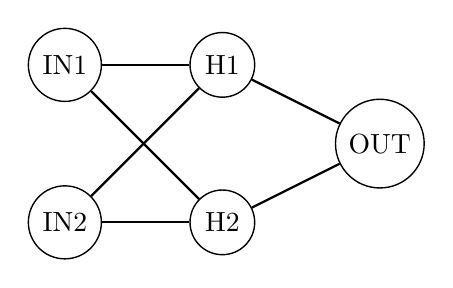
\begin{tikzpicture}
\SetGraphUnit{2}
\GraphInit[vstyle=Normal]
\Vertex[x=2,y=4]{IN1}
\Vertex[x=2,y=2]{IN2}
\Vertex[x=4,y=4]{H1}
\Vertex[x=4,y=2]{H2}
\Vertex[x=6,y=3]{OUT}
\Edges(IN1,H1,OUT)
\Edges(IN1,H2)
\Edges(IN2,H2,OUT)
\Edges(IN2,H1)
\end{tikzpicture}
\\*
\\
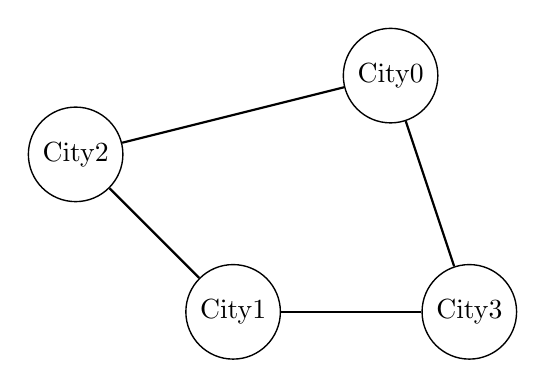
\begin{tikzpicture}
\SetGraphUnit{2}
\GraphInit[vstyle=Normal]
\Vertex[x=6,y=5]{City0}
\Vertex[x=4,y=2]{City1}
\Vertex[x=2,y=4]{City2}
\Vertex[x=7,y=2]{City3}
\Edges(City2,City1)
\Edges(City1,City3)
\Edges(City3,City0)
\Edges(City0,City2)
\end{tikzpicture}
\\*
\\
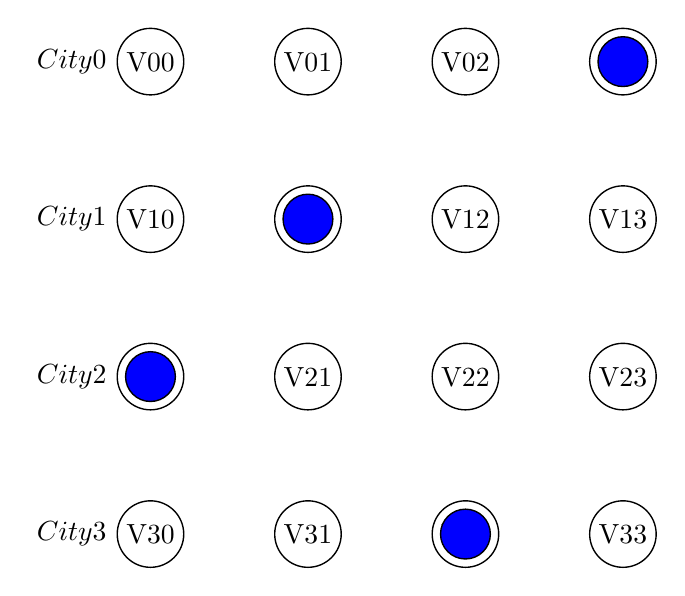
\begin{tikzpicture}
 \newcounter{xp}
 \newcounter{yp}
 \foreach \row in {0,1,2,3}{%
 	\draw (0,-\row*2) node {$City \row$};
 	\foreach \col in {0,1,2,3}{%	
 	  \Vertex[x=1+\col*2,y=-\row*2]{V\row\col}
      }
    }
\AddVertexColor{blue}{V20}
\AddVertexColor{blue}{V03}
\AddVertexColor{blue}{V11}
\AddVertexColor{blue}{V32}
\end{tikzpicture}
\\*
\\
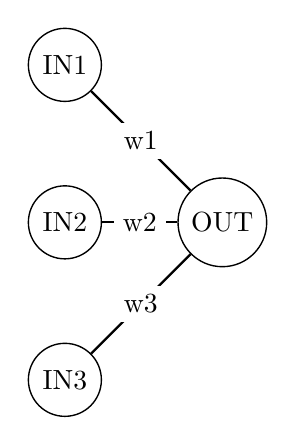
\begin{tikzpicture}
\SetGraphUnit{2}
\GraphInit[vstyle=Normal]
\Vertex[x=2,y=4]{IN1}
\Vertex[x=2,y=2]{IN2}
\Vertex[x=2,y=0]{IN3}
\Vertex[x=4,y=2]{OUT}
\Edges[label=w1](IN1,OUT)
\Edges[label=w2](IN2,OUT)
\Edges[label=w3](IN3,OUT)
\end{tikzpicture}
\end{document}

\\*
\\
\begin{tikzpicture}
\SetGraphUnit{2}
\GraphInit[vstyle=Normal]
\Vertex[x=2,y=0]{IN1}
\Vertex[x=4,y=0]{IN2}
\Vertex[x=6,y=0]{IN3}
\Vertex[x=2,y=2]{H1}
\Vertex[x=4,y=2]{H2}
\Vertex[x=6,y=2]{H3}
\Vertex[x=2,y=4]{OUT1}
\Vertex[x=4,y=4]{OUT1}
\Vertex[x=6,y=4]{OUT1}

\Edges[label=w1](IN1,H1)
\Edges[label=w2](IN1,H2)
\Edges[label=w3](IN1,H3)
\Edges[label=w1](IN2,H1)
\Edges[label=w2](IN2,H2)
\Edges[label=w3](IN2,H3)
\Edges[label=w1](IN3,H1)
\Edges[label=w2](IN3,H2)
\Edges[label=w3](IN3,H3)

\Edges[label=w1](H1,OUT1)
\Edges[label=w2](H1,OUT2)
\Edges[label=w3](H1,OUT3)
\Edges[label=w1](H2,OUT1)
\Edges[label=w2](H2,OUT2)
\Edges[label=w3](H2,OUT3)
\Edges[label=w1](H3,OUT1)
\Edges[label=w2](H3,OUT2)
\Edges[label=w3](H3,OUT3)

\end{tikzpicture}
\end{document}